\chapter{CQRS dan Event Sourcing}
\label{bab:cqrs}

\section*{Tujuan Pembelajaran}

\begin{enumerate}
  \item Menjelaskan pemisahan sisi perintah dari sisi kueri beserta proyeksi
    yang menjembatani keduanya.
  \item Membedakan penyimpanan keadaan sekarang dari penyimpanan event,
    lalu menentukan kapan masing-masing layak dipilih.
  \item Mengukur \textit{write cost} dan \textit{read cost} ketiga versi,
    \textit{replay cost} terhadap panjang \textit{event log}, dan jumlah
    \textit{temporal query} yang terjawab.
\end{enumerate}

\section{Pendahuluan}

Bab-bab sebelumnya memakai satu model data untuk dua pekerjaan yang berbeda.
Tabel kurs pada Bab~2 ditulis lewat bentuk yang sama dengan yang
dipakai membacanya, dan adapter pada Bab~4 pun menyimpan serta
mengambil dari tabel yang sama. Cara tersebut dikenal sebagai CRUD, yaitu
Create, Read, Update, dan Delete atas satu bentuk data.

Pertanyaan yang jarang diajukan adalah apakah kedua pekerjaan itu memang
menuntut bentuk yang sama. Perintah menuntut keadaan terakhir beserta aturan
bisnisnya, sebab perintah harus tahu apakah permintaannya boleh diterima. Kueri
menuntut bentuk yang siap ditampilkan, dan sering menggabungkan angka dari
beberapa tempat. Kedua tuntutan itu tidak selalu bertemu pada satu bentuk yang
sama.

CQRS, yaitu Command Query Responsibility Segregation, menjawabnya dengan
memisahkan model tulis dari model baca~\cite{fowler2011cqrs,young2010cqrs}.
\textit{Event sourcing} melangkah lebih jauh lagi, yaitu keadaan sekarang tidak
disimpan sama sekali, dan yang disimpan hanya deretan event yang pernah
terjadi~\cite{fowler2005eventsourcing}. Bab ini memakai satu domain kecil yang
punya riwayat, yaitu buku besar saldo dompet mahasiswa, lalu menulisnya tiga
kali dengan perilaku luar yang sama persis. Pembahasannya mengikuti kerangka
yang disusun Richards dan Ford~\cite{richards2020fundamentals}.

\section{Perintah dan Kueri}

Pembagiannya berangkat dari satu aturan lama. \textbf{Perintah} mengubah
keadaan dan tidak mengembalikan data. \textbf{Kueri} mengembalikan data dan
tidak mengubah keadaan apa pun. Aturan itu disebut Command Query Separation
(CQS) dan berlaku pada tingkat metode. CQRS menaikkan pembagian tersebut satu
tingkat, sehingga yang terpisah bukan lagi metodenya, melainkan
modelnya~\cite{fowler2011cqrs}.

Gambar~\ref{fig:satu-dua-model} membandingkan keduanya. Pada susunan atas,
perintah dan kueri bertemu pada satu tabel. Pada susunan bawah, keduanya tidak
pernah menyentuh tabel yang sama.

\begin{figure}[htbp]
  \centering
  \begin{tikzpicture}[
    kotak/.style={draw, rounded corners=2pt, minimum width=2.0cm,
      minimum height=0.85cm, align=center, font=\tiny\bfseries},
    panah/.style={-{Stealth[length=2mm]}, thick}
  ]
    \node[kotak, fill=gray!22] (kirim1) {Perintah\\
      {\tiny\mdseries setor, bayar}};
    \node[kotak, fill=praditagreen!25, right=0.7cm of kirim1] (tabel1)
      {dompet\\{\tiny\mdseries satu baris keadaan}};
    \node[kotak, fill=gray!22, right=0.7cm of tabel1] (baca1) {Kueri\\
      {\tiny\mdseries berapa saldo}};
    \node[left=0.25cm of kirim1, font=\scriptsize\bfseries] {CRUD};

    \node[kotak, fill=gray!22, below=1.3cm of kirim1] (kirim2) {Perintah\\
      {\tiny\mdseries setor, bayar}};
    \node[kotak, fill=blue!8, right=0.45cm of kirim2] (tulis)
      {dompet\_tulis\\{\tiny\mdseries model tulis}};
    \node[kotak, fill=praditagreen!15, right=0.45cm of tulis] (proyeksi)
      {terapkan()\\{\tiny\mdseries proyeksi}};
    \node[kotak, fill=green!10, right=0.45cm of proyeksi] (bacamodel)
      {ringkasan\_baca\\{\tiny\mdseries model baca}};
    \node[kotak, fill=gray!22, right=0.45cm of bacamodel] (baca2) {Kueri\\
      {\tiny\mdseries berapa saldo}};
    \node[left=0.25cm of kirim2, font=\scriptsize\bfseries] {CQRS};

    \draw[panah] (kirim1) -- (tabel1);
    \draw[panah] (baca1) -- (tabel1);
    \draw[panah] (kirim2) -- (tulis);
    \draw[panah] (tulis) -- (proyeksi);
    \draw[panah] (proyeksi) -- (bacamodel);
    \draw[panah] (baca2) -- (bacamodel);
  \end{tikzpicture}
  \caption{Satu model dibanding dua model. Pada susunan bawah, kueri berhenti
    di model baca, dan bentuk model baca itu bebas mengikuti pertanyaannya}
  \label{fig:satu-dua-model}
\end{figure}

Analogi yang mendekati adalah loket pembayaran uang kuliah. Mahasiswa yang
membayar mengantre di loket keuangan, lalu petugasnya memeriksa tagihan,
menerima uang, dan mencatatnya. Mahasiswa yang hanya ingin tahu sisa tagihannya
tidak ikut antrean itu, sebab angkanya sudah tertera di portal. Loket dan
portal bukan tempat yang sama, walaupun angkanya berasal dari catatan yang
sama. Perbedaan yang penting, portal diperbarui sesudah loket mencatat, bukan
pada saat yang sama persis.

Tabel~\ref{tab:sisi-perintah-kueri} merangkum tanggung jawab dan larangan
ketiga bagiannya.

\begin{table}[htbp]
  \centering
  \caption{Tanggung jawab dan larangan sisi perintah, proyeksi, dan sisi kueri}
  \label{tab:sisi-perintah-kueri}
  \begin{tabularx}{\textwidth}{|l|X|X|}
    \hline
    \textbf{Bagian} & \textbf{Tanggung jawab} & \textbf{Tidak boleh mengerjakan} \\
    \hline
    Sisi perintah & Memeriksa aturan bisnis lalu menyimpan perubahannya & Menyusun bentuk tampilan, dan melayani kueri \\
    \hline
    Proyeksi & Melipat perubahan yang diterima ke atas model baca & Menolak perubahan, sebab perubahannya sudah terjadi \\
    \hline
    Sisi kueri & Membaca model baca lalu menyerahkannya apa adanya & Menyentuh model tulis, dan mengubah nilai apa pun \\
    \hline
  \end{tabularx}
\end{table}

Pemisahan itu punya dua konsekuensi praktis. Pertama, bentuk model baca bebas
mengikuti pertanyaan yang akan datang, sebab aturan bisnis tidak lagi
membebaninya. Kedua, model baca dapat tertinggal dari model tulis, sebab
pembaruannya terjadi sesudah perintah selesai. Konsekuensi kedua itulah yang
menimbulkan persoalan berikutnya. Pertanyaannya, siapa yang memperbarui model
baca, dan seberapa lama tertinggalnya.

\section{Proyeksi yang Menjembatani Dua Model}

Penjembatannya disebut \textbf{proyeksi}, yaitu fungsi yang melipat satu
perubahan ke atas ringkasan yang sudah ada. Masukannya ringkasan lama beserta
perubahan yang baru diterima, sedangkan keluarannya ringkasan baru. Fungsi
seperti itu tidak menyimpan apa pun sendiri, sehingga hasilnya mudah diuji dan
mudah dijalankan ulang.

Ketiga versi bab ini memenuhi kontrak yang sama, dan kontraknya berada di
\berkas{sources/chapter10/domain.py}. Listing~\ref{lst:kontrak-cqrs}
memperlihatkan bagian terpentingnya, yaitu metode yang dipanggil seluruh skrip
pengukuran.

\begin{lstlisting}[style=PythonStyle, caption={Perilaku luar yang wajib sama
  pada ketiga versi, tersedia di \berkas{sources/chapter10/domain.py}},
  label=lst:kontrak-cqrs]
class BukuBesar(Protocol):
  """Perilaku luar yang wajib sama pada ketiga versi penyimpanan."""

  def jalankan(self, perintah: Perintah) -> int:
    """Menjalankan satu perintah lalu mengembalikan int berisi saldo baru."""

  def baca_saldo(self, pemilik: str) -> int:
    """Mengembalikan int berisi saldo sekarang milik pemilik tersebut."""

  def jawab_saldo_pada(self, pemilik: str, batas_waktu: str) -> Jawaban:
    """Mengembalikan Jawaban berisi saldo pada waktu yang diminta."""
\end{lstlisting}

Versi CQRS menulis dua kali untuk setiap perintah yang diterima. Tulisan
pertama masuk ke model tulis, sedangkan tulisan kedua masuk ke model baca lewat
proyeksi. Listing~\ref{lst:jalankan-cqrs} memperlihatkan keduanya berurutan.

\begin{lstlisting}[style=PythonStyle, caption={Satu perintah menulis dua kali,
  tersedia di \berkas{sources/chapter10/versi_cqrs.py}}, label=lst:jalankan-cqrs]
saldo_lama = baris[0] if baris else 0
saldo_baru = domain.periksa_perintah(saldo_lama, perintah)
self.koneksi.execute(
  "INSERT INTO dompet_tulis (pemilik, saldo) VALUES (?, ?) "
  "ON CONFLICT(pemilik) DO UPDATE SET saldo = excluded.saldo",
  (perintah.pemilik, saldo_baru),
)
self.koneksi.commit()
if self.proyeksi_langsung:
  self.proyeksikan(perintah)
else:
  self.antrean.append(perintah)
return saldo_baru
\end{lstlisting}

Gambar~\ref{fig:sekuens-cqrs} menyandingkan urutan kedua versi untuk satu
perintah yang diikuti satu kueri. Perhatikan bahwa jalur kueri pada versi CQRS
berhenti di model baca.

\begin{figure}[htbp]
  \centering
  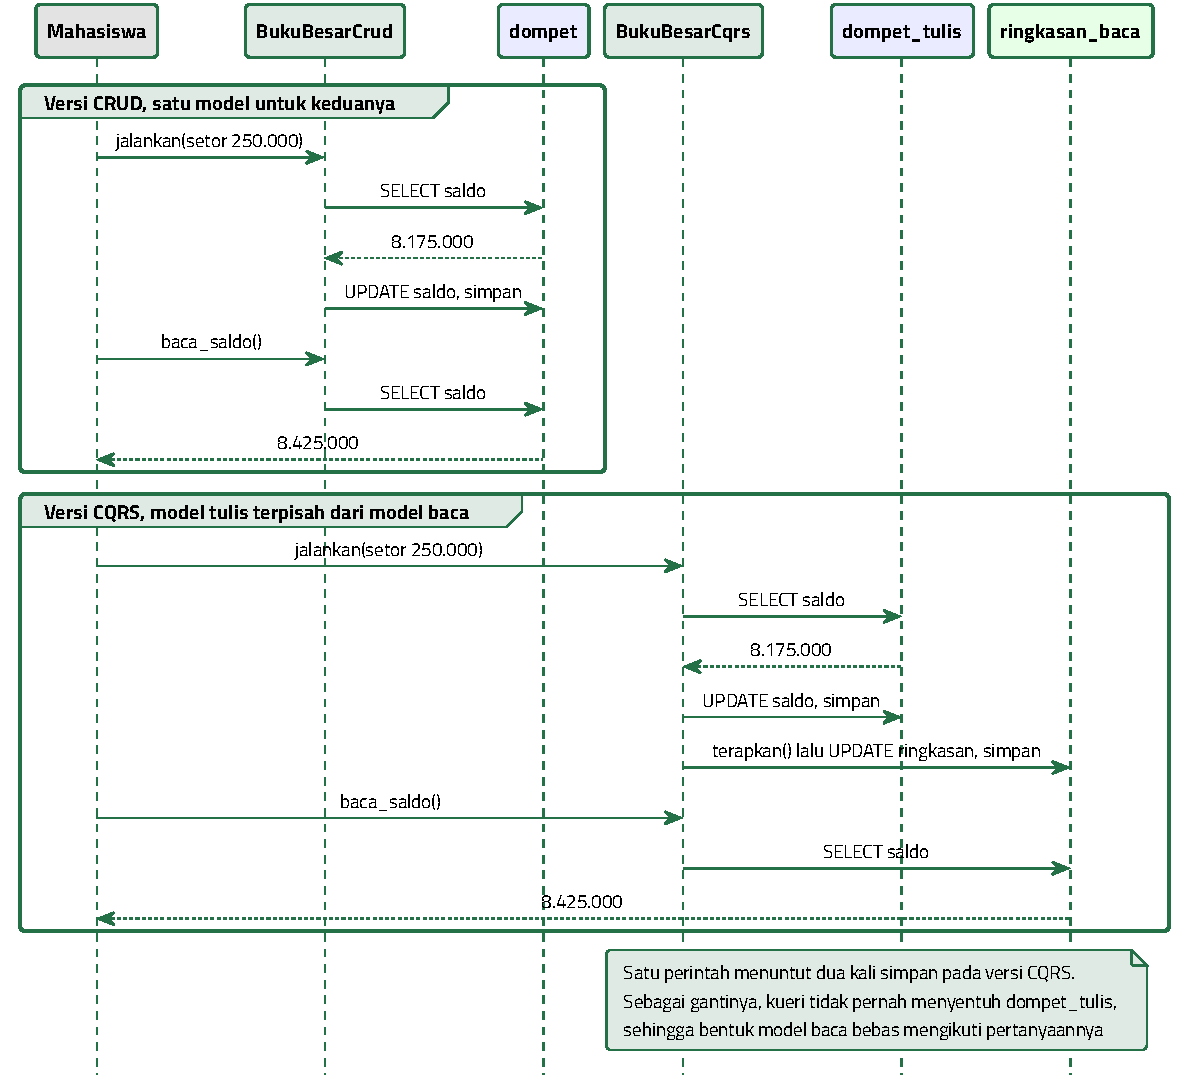
\includegraphics[width=\textwidth, height=0.52\textheight,
    keepaspectratio]{sekuens-cqrs.pdf}
  \caption{Satu perintah lalu satu kueri pada kedua versi. Versi CQRS menyimpan
    dua kali, sedangkan kuerinya tidak pernah menyentuh model tulis}
  \label{fig:sekuens-cqrs}
\end{figure}

Percabangan \texttt{if} pada Listing~\ref{lst:jalankan-cqrs} menyimpan pilihan
yang menentukan. Bila proyeksinya dijalankan langsung, model baca selalu
sejalan dengan model tulis. Bila proyeksinya ditunda, model baca tertinggal
sampai antreannya didorong. Keadaan itulah yang dikenal sebagai konsistensi
yang menyusul, atau \textit{eventual consistency}~\cite{microsoft2024cqrs}.
Menjalankan
\texttt{python versi\_cqrs.py} memperlihatkan jaraknya dengan angka. Model baca
masih menunjukkan saldo nol padahal sembilan puluh lima perubahan sudah
diterima model tulis, dan barulah sesudah antreannya didorong angkanya menjadi
8.425.000 rupiah.

Contoh bab ini menjalankan proyeksinya langsung, agar hasil latihan dapat
diulang. Pilihan itu membuat latensi tulisnya naik, dan kenaikannya diukur pada
seksi berikutnya.

\section{Menyimpan Event, Bukan Keadaan}

Pemisahan model belum menyentuh persoalan yang berbeda, yaitu nilai lama yang
hilang. Baik versi CRUD maupun versi CQRS sama-sama menimpa baris saldonya,
sehingga nilai sebelumnya tidak tersisa. \textit{Event sourcing} menolak
penimpaan itu. Yang disimpan hanya \textbf{event}, yaitu fakta bahwa
sesuatu telah terjadi, dan keadaan sekarang dihitung ulang dengan melipat
seluruh event tersebut~\cite{fowler2005eventsourcing}.

Gambar~\ref{fig:event-log} menunjukkan enam event pertama pada contoh
bab ini beserta saldo yang terbentuk sesudah masing-masing event.

\begin{figure}[htbp]
  \centering
  \begin{tikzpicture}[
    event/.style={draw, rounded corners=2pt, minimum width=1.55cm,
      minimum height=0.8cm, align=center, font=\tiny\bfseries},
    hasil/.style={font=\tiny, align=center},
    panah/.style={-{Stealth[length=2mm]}, thick}
  ]
    \node[event, fill=blue!8] (e1) {setor\\
      {\tiny\mdseries +307.000}};
    \node[event, fill=blue!8, right=0.14cm of e1] (e2) {bayar\\
      {\tiny\mdseries -175.000}};
    \node[event, fill=blue!8, right=0.14cm of e2] (e3) {bayar\\
      {\tiny\mdseries -36.000}};
    \node[event, fill=blue!8, right=0.14cm of e3] (e4) {setor\\
      {\tiny\mdseries +51.000}};
    \node[event, fill=blue!8, right=0.14cm of e4] (e5) {bayar\\
      {\tiny\mdseries -38.000}};
    \node[event, fill=green!10, right=0.14cm of e5] (e6) {setor\\
      {\tiny\mdseries +100.000}};
    \node[right=0.14cm of e6, font=\tiny] (lanjut) {\dots};

    \node[hasil, below=0.12cm of e1] {307.000};
    \node[hasil, below=0.12cm of e2] {132.000};
    \node[hasil, below=0.12cm of e3] {96.000};
    \node[hasil, below=0.12cm of e4] {147.000};
    \node[hasil, below=0.12cm of e5] {109.000};
    \node[hasil, below=0.12cm of e6] {209.000};

    \node[event, fill=praditagreen!25, minimum width=3.4cm,
      below=0.95cm of e5] (snap) {snapshot\\
      {\tiny\mdseries urutan 6, saldo 209.000}};
    \draw[panah, dashed] (snap) -- (e6);
    \node[below=0.12cm of snap, font=\tiny, align=center]
      {penghitungan ulang berikutnya melanjutkan dari sini};
  \end{tikzpicture}
  \caption{Enam event pertama beserta saldo sesudah masing-masing. Angka
    saldo di bawahnya tidak disimpan, melainkan dihitung ulang setiap kali
    dibutuhkan}
  \label{fig:event-log}
\end{figure}

Perhatikan satu hal yang tidak tampak pada gambar tersebut. Perintah keempat
sampai kedelapan pada deretan aslinya berupa pembayaran yang melebihi saldo,
dan kelimanya ditolak. Penolakan bukan event, sehingga tidak satu pun
meninggalkan baris pada log. \textit{Event log} memuat yang terjadi, bukan yang
diminta.

Listing~\ref{lst:jalankan-event} memperlihatkan jalur perintahnya. Saldo untuk
memeriksa aturan bisnis disusun ulang lebih dahulu, sebab tidak ada kolom saldo
yang dapat dibaca langsung.

\begin{lstlisting}[style=PythonStyle, caption={Perintah menambah baris, bukan
  menimpa baris, tersedia di \berkas{sources/chapter10/versi_event.py}},
  label=lst:jalankan-event]
def jalankan(self, perintah: domain.Perintah) -> int:
  """Menambah satu baris event sesudah aturan bisnisnya dipenuhi."""
  _, ringkasan = self.susun_ringkasan(perintah.pemilik)
  saldo_baru = domain.periksa_perintah(ringkasan.saldo, perintah)
  self.koneksi.execute(
    "INSERT INTO event (pemilik, jenis, nominal, waktu) "
    "VALUES (?, ?, ?, ?)",
    (perintah.pemilik, perintah.jenis, perintah.nominal, perintah.waktu),
  )
  self.koneksi.commit()
  return saldo_baru
\end{lstlisting}

Gambar~\ref{fig:kelas-cqrs} menunjukkan hubungan keempat bagiannya sebagai
diagram kelas. Panahnya berjalan satu arah, yaitu dari perintah menuju
\textit{event log}, lalu dari \textit{event log} menuju model baca lewat
proyeksi.

\begin{figure}[htbp]
  \centering
  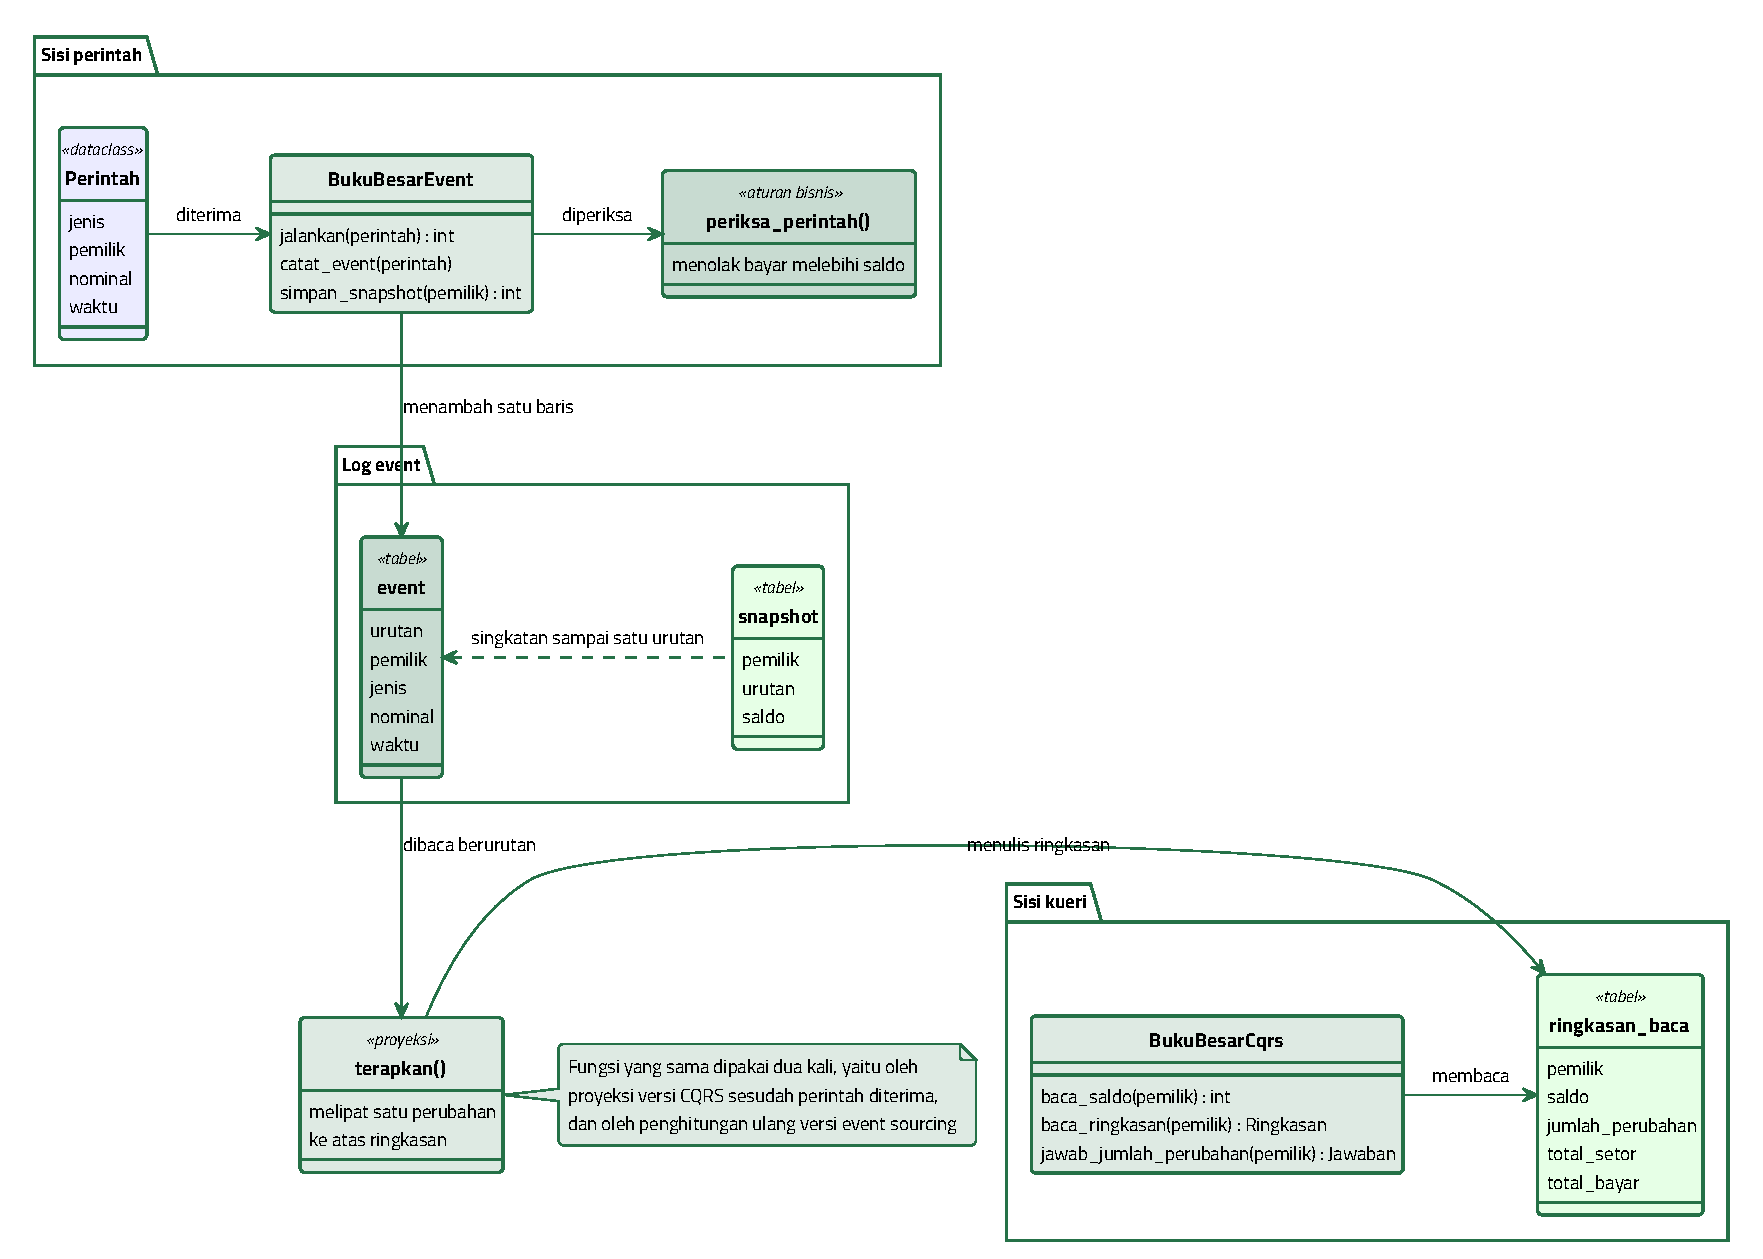
\includegraphics[width=\textwidth, height=0.72\textheight,
    keepaspectratio]{kelas-cqrs.pdf}
  \caption{Sisi perintah, \textit{event log}, proyeksi, dan sisi kueri. Fungsi
    \texttt{terapkan()} yang sama dipakai proyeksi versi CQRS dan penghitungan
    ulang versi \textit{event sourcing}}
  \label{fig:kelas-cqrs}
\end{figure}

Susunan itu membalik satu kebiasaan lama. Pada versi CRUD, menulis itu murah
sedangkan riwayat itu mahal, sebab riwayatnya memang tidak ada. Pada versi
\textit{event sourcing}, menulis tetap murah sedangkan membaca menjadi mahal,
sebab setiap pembacaan menuntut penghitungan ulang. Pertanyaannya, seberapa
mahal penghitungan ulang itu sebenarnya.

\section{Biaya Tulis dan Biaya Baca}

Dua angka diukur di seksi ini. Biaya menjalankan satu perintah disebut
\textit{write cost}, sedangkan biaya menjawab satu kueri disebut
\textit{read cost}. Keduanya dihitung \texttt{ukur\_latensi.py}, yaitu seratus
perintah disusul seratus kueri pada ketiga versi. Setiap perintah dan setiap
kueri diukur sendiri-sendiri, sehingga yang dilaporkan sebaran seratus angka.
Versi \textit{event sourcing} dijalankan tanpa snapshot di sini, sehingga
setiap kueri melipat seluruh \textit{event log}.

Tabel~\ref{tab:latensi} memuat hasil satu kali pengukuran nyata. Ketiga versi
berakhir pada saldo yang sama, yaitu 8.425.000 rupiah, sehingga perbedaannya
benar-benar berasal dari cara penyimpanannya.

\begin{table}[htbp]
  \centering
  \caption{Latensi tulis dan latensi baca ketiga versi, seratus perintah dan
    seratus kueri}
  \label{tab:latensi}
  \begin{tabularx}{\textwidth}{|X|l|l|l|}
    \hline
    \textbf{Yang diukur} & \textbf{Median} & \textbf{Persentil ke-95} & \textbf{Terbesar} \\
    \hline
    Tulis CRUD & 2,1958 ms & 2,6481 ms & 3,2731 ms \\
    \hline
    Tulis CQRS & 4,6257 ms & 5,4658 ms & 7,8009 ms \\
    \hline
    Tulis \textit{event sourcing} & 2,5998 ms & 2,9981 ms & 3,4557 ms \\
    \hline
    Baca CRUD & 0,0695 ms & 0,1249 ms & 0,1472 ms \\
    \hline
    Baca CQRS & 0,0726 ms & 0,0835 ms & 0,1047 ms \\
    \hline
    Baca \textit{event sourcing} & 0,3078 ms & 0,4598 ms & 0,5240 ms \\
    \hline
  \end{tabularx}
\end{table}

Angka pada baris kedua itu janggal bila dibaca sekilas. Versi CQRS justru
menulis paling lambat, padahal pemisahan model sering dijual sebagai cara
mempercepat. Sebabnya sederhana, yaitu satu perintah menuntut dua kali simpan
ke cakram, sekali untuk model tulis dan sekali untuk model baca. Selisihnya
2,4299 milidetik, yaitu 1,1 kali latensi tulis versi CRUD seluruhnya.

Ada pula kejanggalan kedua yang layak dicatat. \textit{Range} di dalam jalur
CRUD sendiri tercatat 3,1666 milidetik, yaitu 1,3 kali selisih yang dicari.
Menurut ukuran Bab~2, selisih sebesar itu belum dapat disebut
ada. Pencacahan per putaran justru menunjuk arah yang tegas, yaitu versi CQRS
lebih lambat pada 99 dari 100 perintah. Dua ukuran itu tidak sejalan, dan yang
lebih peka di sini adalah pencacahannya, sebab satu perintah lambat sudah cukup
melebarkan \textit{range} tanpa mengubah siapa yang menang pada tiap putaran.

Sisi bacanya memberi gambaran yang jauh lebih bersih. Versi \textit{event
sourcing} membaca 0,2353 milidetik lebih lambat daripada versi CQRS, sedangkan
\textit{range} di dalam jalur CQRS hanya 0,0337 milidetik, yaitu 0,1 kali
selisihnya. Pencacahan per kueri menegaskannya dengan angka 100 dari 100.
Selisih yang seperti inilah yang layak dilaporkan.

\section{Snapshot dan Penghitungan Ulang}

Latensi baca sebesar itu masih ringan, sebab lognya baru berisi sembilan puluh
lima event. Pertanyaan yang sesungguhnya adalah apa yang terjadi ketika
lognya berisi ratusan ribu baris. Biaya melipat ulang seluruh log itu disebut
\textit{replay cost}, dan besarnya diukur
\texttt{ukur\_penghitungan\_ulang.py} pada tiga panjang log, yaitu seribu,
sepuluh ribu, dan seratus ribu event.

Penawarnya disebut \textbf{snapshot}, yaitu hasil lipatan sampai satu nomor
urut tertentu yang ikut disimpan. Penghitungan berikutnya cukup memuat snapshot
lalu melanjutkan dari sana. Snapshot bukan sumber kebenaran, melainkan
singkatan, dan singkatan itu boleh dibuang lalu dibentuk ulang kapan saja.

Analogi yang mendekati adalah buku besar tulis tangan di koperasi kampus.
Setiap transaksi ditulis pada baris baru, dan tidak ada baris yang dihapus.
Saldo akhir halaman ditulis di bagian bawah setiap halaman, sehingga petugas
halaman berikutnya tidak perlu menjumlah dari halaman pertama. Angka di bawah
halaman itulah snapshotnya. Bila angkanya diragukan, seluruh baris masih ada
dan dapat dijumlah ulang.

Listing~\ref{lst:titik-mulai} memperlihatkan bagaimana snapshot dipakai. Bila
belum ada snapshot, penghitungan mulai dari nomor urut nol, yaitu dari
event pertama.

\begin{lstlisting}[style=PythonStyle, caption={Snapshot menentukan dari mana
  lipatan dimulai, tersedia di \berkas{sources/chapter10/versi_event.py}},
  label=lst:titik-mulai]
def titik_mulai(self, pemilik: str) -> tuple[int, domain.Ringkasan]:
  """Menentukan dari mana penghitungan ulang layak dimulai."""
  if not self.pakai_snapshot:
    return 0, domain.RINGKASAN_KOSONG
  kursor = self.koneksi.execute(
    "SELECT urutan, saldo, jumlah_perubahan, total_setor, total_bayar, "
    "waktu_terakhir FROM snapshot WHERE pemilik = ?", (pemilik,)
  )
  baris = kursor.fetchone()
  if not baris:
    return 0, domain.RINGKASAN_KOSONG
  return baris[0], domain.Ringkasan(*baris[1:])
\end{lstlisting}

Snapshot pada pengukuran ini sengaja dipasang sebelum dua ratus lima puluh
event terakhir. Jalur bersnapshot karena itu selalu punya dua ratus lima
puluh event untuk dilipat, berapa pun panjang lognya.
Tabel~\ref{tab:penghitungan-ulang} memuat hasilnya.

\begin{table}[htbp]
  \centering
  \caption{Waktu menyusun ulang model baca dari \textit{event log}, seratus putaran
    untuk setiap keadaan}
  \label{tab:penghitungan-ulang}
  \begin{tabularx}{\textwidth}{|X|l|l|l|}
    \hline
    \textbf{Yang diukur} & \textbf{Median} & \textbf{Persentil ke-95} & \textbf{Terbesar} \\
    \hline
    Tanpa snapshot, 1.000 event & 1,9146 ms & 2,5361 ms & 3,2533 ms \\
    \hline
    Dengan snapshot, 1.000 event & 0,7147 ms & 0,7882 ms & 0,9063 ms \\
    \hline
    Tanpa snapshot, 10.000 event & 17,1736 ms & 28,0888 ms & 32,7969 ms \\
    \hline
    Dengan snapshot, 10.000 event & 0,6083 ms & 0,7103 ms & 0,8785 ms \\
    \hline
    Tanpa snapshot, 100.000 event & 173,9364 ms & 602,7324 ms & 781,6385 ms \\
    \hline
    Dengan snapshot, 100.000 event & 2,9440 ms & 4,4089 ms & 7,7233 ms \\
    \hline
  \end{tabularx}
\end{table}

Tiga hal terbaca dari tabel tersebut. Pertama, jalur tanpa snapshot tumbuh
sejalan dengan panjang lognya, yaitu dari 1,9146 menjadi 173,9364 milidetik
ketika lognya seratus kali lebih panjang. Kedua, jalur bersnapshot hampir
tidak bergantung pada panjang log, yaitu 0,7147 milidetik pada seribu event,
0,6083 milidetik pada sepuluh ribu, lalu 2,9440 milidetik pada seratus ribu.
Kenaikan terakhir itu datang dari penelusuran indeks yang memang lebih dalam
pada tabel yang lebih besar, dan besarnya 4,1 kali, sedangkan jalur tanpa
snapshot naik 90,8 kali pada rentang yang sama. Ketiga, saldo kedua jalur
selalu sama, sehingga snapshot benar-benar hanya singkatan.

Satu angka pada tabel itu janggal dan perlu dijelaskan. Persentil ke-95 jalur
tanpa snapshot pada seratus ribu event mencapai 602,7324 milidetik, yaitu
3,5 kali mediannya sendiri. Ekor selebar itu tidak muncul pada jalur
bersnapshot. Sebabnya adalah jumlah objek sementara yang dibuat selama lipatan,
yaitu seratus ribu objek \texttt{Ringkasan} pada setiap putaran. Pemungut
sampah Python bekerja pada sebagian putaran, dan putaran itulah yang menjadi
ekornya. Gejala seperti ini hanya terlihat bila persentil dan nilai terbesar
ikut dilaporkan.

\section{Harga Penyimpanan dan Pertanyaan yang Terjawab}

Riwayat yang lengkap tidak diperoleh dengan gratis. Skrip
\texttt{ukur\_penyimpanan.py} menjalankan sepuluh ribu perintah yang sama pada
ketiga versi, lalu membaca ukuran berkas basis datanya.
Tabel~\ref{tab:penyimpanan} memuat hasilnya.

\begin{table}[htbp]
  \centering
  \caption{Besar berkas sesudah sepuluh ribu perintah, 9.995 di antaranya
    diterima}
  \label{tab:penyimpanan}
  \begin{tabularx}{\textwidth}{|l|l|X|}
    \hline
    \textbf{Versi} & \textbf{Ukuran berkas} & \textbf{Isinya} \\
    \hline
    CRUD & 12,0 KiB & 1 baris keadaan \\
    \hline
    CQRS & 20,0 KiB & 2 baris keadaan, yaitu model tulis dan model baca \\
    \hline
    \textit{Event sourcing} & 668,0 KiB & 9.995 baris event beserta snapshotnya \\
    \hline
  \end{tabularx}
\end{table}

Berkas lognya 55,7 kali lebih besar daripada berkas keadaan, dan setiap
event menghabiskan sekitar 68 bita. Angka itu tumbuh selama sistemnya
hidup, sedangkan berkas keadaan berhenti tumbuh sejak baris pertamanya
tertulis. Pertanyaannya, apa yang dibeli dengan ruang sebesar itu.

Jawabannya adalah pertanyaan yang dapat dijawab. Skrip
\texttt{tanya\_riwayat.py} mengajukan dua pertanyaan kepada ketiga versi.
Pertanyaan pertama menyangkut keadaan pada satu titik waktu di masa lampau,
atau \textit{temporal query}, yaitu berapa saldo pada 1 Maret 2026 pukul 08.30.
Pertanyaan kedua menyangkut jumlah perubahan, yaitu berapa kali saldo pernah
berubah. Tabel~\ref{tab:pertanyaan} memuat jawabannya.

\begin{table}[htbp]
  \centering
  \caption{Dua pertanyaan riwayat yang diajukan kepada ketiga versi}
  \label{tab:pertanyaan}
  \begin{tabularx}{\textwidth}{|l|X|X|}
    \hline
    \textbf{Versi} & \textbf{Saldo pada 08.30} & \textbf{Jumlah perubahan} \\
    \hline
    CRUD & tidak terjawab & tidak terjawab \\
    \hline
    CQRS & tidak terjawab & 95 \\
    \hline
    \textit{Event sourcing} & 2.132.000 & 95 \\
    \hline
  \end{tabularx}
\end{table}

Baris tengah tabel itu yang paling menarik. Versi CQRS mampu menjawab
pertanyaan kedua, sebab proyeksinya memang menyimpan pencacah perubahan sejak
awal. Versi CQRS tetap tidak mampu menjawab pertanyaan pertama, sebab model
bacanya satu baris per pemilik dan baris itu ditimpa terus-menerus. Model baca
hanya menjawab pertanyaan yang sudah diduga saat merancangnya, sedangkan
\textit{event log} menjawab pertanyaan yang belum terpikirkan sekalipun.

Kasus berikut memperlihatkan harga ketidakmampuan tersebut. Sebuah unit
keuangan kampus menjalankan dompet mahasiswa di atas satu tabel keadaan. Pada
suatu malam, pekerjaan pemotongan tagihan berjalan dua kali karena percobaan
ulang yang gagal terdeteksi. Keesokan paginya keluhan mulai masuk, dan
pimpinan menanyakan dua hal, yaitu mahasiswa mana saja yang terpotong dua kali
dan berapa saldo mereka sebelum pemotongan. Tabelnya hanya memuat saldo
terakhir, sehingga kedua pertanyaan itu tidak terjawab dari sistem. Unit
tersebut akhirnya meminta bukti transfer dari mahasiswa satu per satu, lalu
mencocokkannya dengan tangan selama dua minggu. Yang mahal ternyata bukan
kesalahan programnya, melainkan ketiadaan bahan untuk menjawabnya.

\section{Ringkasan}

CQRS memisahkan model yang dipakai menulis dari model yang dipakai membaca.
Perintah memeriksa aturan bisnis lalu menyimpan perubahannya, sedangkan kueri
membaca model yang bentuknya mengikuti pertanyaan. Penjembatannya proyeksi,
yaitu fungsi yang melipat satu perubahan ke atas ringkasan yang sudah ada.
Fungsi pelipat itu pula yang dipakai \textit{event sourcing} ketika menghitung
ulang keadaannya.

Pemisahan tersebut tidak gratis. Satu perintah pada versi CQRS menuntut dua
kali simpan, dan latensi tulisnya tercatat 4,6257 milidetik melawan 2,1958
milidetik pada versi CRUD. Sisi bacanya nyaris tidak berbeda selama
pertanyaannya masih sesederhana berapa saldo sekarang. Keuntungan pemisahan
baru terasa ketika bentuk pertanyaannya jauh dari bentuk penyimpanannya.

\textit{Event sourcing} menjawab persoalan yang berbeda, yaitu riwayat yang
hilang karena penimpaan. Yang disimpan hanya event, dan keadaan sekarang
dihitung ulang dari event itu. Harganya terbaca pada dua tempat, yaitu
latensi baca yang naik menjadi 0,3078 milidetik dan berkas yang membengkak
menjadi 55,7 kali berkas keadaan. Penghitungan ulang yang panjang ditekan
dengan snapshot, dan pada seratus ribu event snapshot mempercepatnya 59,1
kali.

Yang dibeli dengan harga tersebut adalah pertanyaan yang dapat dijawab. Versi
CRUD tidak menjawab satu pun dari dua pertanyaan riwayat pada bab ini. Versi
CQRS menjawab satu, yaitu pertanyaan yang sudah diduga saat proyeksinya
dirancang. Versi \textit{event sourcing} menjawab keduanya, termasuk pertanyaan
yang belum terpikirkan ketika penyimpanannya dirancang.

Pesan utama bab ini karena itu bukan bahwa penimpaan selalu keliru, melainkan
bahwa penimpaan adalah keputusan yang harus disadari. Menimpa satu baris berarti
memilih kemurahan tulis dan membuang riwayat. Selama pertanyaan yang datang
hanya menyangkut keadaan sekarang, pilihan itu tetap benar, dan bab ini
menyediakan angkanya untuk menimbang kapan pilihan itu berhenti benar.

\section{Latihan}

Ketiga latihan berikut memakai satu basis kode yang sama di
\berkas{sources/chapter10/}, tetapi menyasar tiga masalah yang berbeda.
Latihan~1 mengukur \textit{write cost} dan \textit{read cost} ketiga versi.
Latihan~2 mengukur \textit{replay cost} terhadap panjang \textit{event log}.
Latihan~3 mengajukan \textit{temporal query} kepada ketiganya. Hasil setiap
mahasiswa dapat
berbeda, dan yang dilaporkan adalah pola perbandingannya, bukan angka
mutlaknya.

Venv yang sama dipakai kembali, dan pengaktifannya seperti pada
Listing~\ref{lst:venv-ch10}. Bab ini hanya memakai pustaka standar Python,
termasuk \texttt{sqlite3}, sehingga tidak ada pemasangan tambahan.

\begin{lstlisting}[language=bash, caption={Menyiapkan bahan sebelum ketiga
  latihan, skrip tersedia di \berkas{sources/siapkan_venv.sh}},
  label=lst:venv-ch10]
bash sources/siapkan_venv.sh
source .venv/bin/activate
cd sources/chapter10
python versi_event.py
# Keluarannya baris kedua: Event tersimpan    : 95
\end{lstlisting}

\subsection*{Latihan 1: \textit{Write Cost} dan \textit{Read Cost}}

Latihan ini menguji dugaan yang sering diucapkan tanpa angka, yaitu pemisahan
model membuat sistem lebih cepat. Dugaan itu menyebut angka, sehingga dapat
dibuktikan salah. Langkah kerjanya sebagai berikut.

\begin{enumerate}
  \item Jalankan perintah pada Listing~\ref{lst:jalankan-latensi10}, lalu catat
    baris \texttt{Saldo akhir ketiga versi} untuk memastikan ketiganya berakhir
    sama.
  \item Catat keenam baris latensi beserta median, persentil ke-95, dan nilai
    terbesarnya.
  \item Catat ketiga blok pembanding di bagian bawah laporan, terutama baris
    \texttt{Rentang dibagi selisih}.
  \item Buka \berkas{sources/chapter10/versi_cqrs.py}, lalu hitung berapa kali
    \texttt{commit} dipanggil untuk satu perintah.
  \item Ubah \texttt{JUMLAH\_PERINTAH} menjadi 500, jalankan ulang, lalu catat
    perubahan pada latensi baca versi \textit{event sourcing}.
\end{enumerate}

\begin{lstlisting}[language=bash, caption={Mengukur \textit{write cost} dan
  \textit{read cost}, skrip tersedia di
  \berkas{sources/chapter10/ukur_latensi.py}}, label=lst:jalankan-latensi10]
python ukur_latensi.py
# Keluarannya: Saldo akhir ketiga versi : 8425000 (sama)
#              tulis CRUD   median 2.1958 ms  p95 2.6481  tbsr 3.2731
#              tulis CQRS   median 4.6257 ms  p95 5.4658  tbsr 7.8009
#              baca  event  median 0.3078 ms  p95 0.4598  tbsr 0.5240
#              Tulis CQRS lebih lambat   : 99 dari 100
#              Baca event lebih lambat   : 100 dari 100
\end{lstlisting}

Tabel~\ref{tab:lat1cqrs-contoh} berisi hasil satu kali pengukuran nyata.

\begin{table}[htbp]
  \centering
  \caption{Contoh hasil Latihan 1 yang sudah terisi, seratus perintah dan
    seratus kueri}
  \label{tab:lat1cqrs-contoh}
  \begin{tabularx}{\textwidth}{|X|l|l|}
    \hline
    \textbf{Yang dilaporkan} & \textbf{Tulis} & \textbf{Baca} \\
    \hline
    Median CRUD & 2,1958 ms & 0,0695 ms \\
    \hline
    Median CQRS & 4,6257 ms & 0,0726 ms \\
    \hline
    Median \textit{event sourcing} & 2,5998 ms & 0,3078 ms \\
    \hline
    Persentil ke-95 \textit{event sourcing} & 2,9981 ms & 0,4598 ms \\
    \hline
    \textit{Range} dibagi selisih & 1,3 kali & 0,1 kali \\
    \hline
    Putaran versi kedua lebih lambat & 99 dari 100 & 100 dari 100 \\
    \hline
  \end{tabularx}
\end{table}

Baris kelima pada kedua kolom itu menunjuk arah yang berbeda, dan perbedaannya
disengaja. Pada sisi tulis, \textit{range} di dalam satu versi lebih besar
daripada selisih yang dicari, sehingga selisihnya belum dapat disebut ada
menurut ukuran Bab~2. Pada sisi baca, \textit{range}-nya justru
sepersepuluh selisihnya. Isikan hasil pengukuran pada
Tabel~\ref{tab:lat1cqrs-hasil}.

\begin{table}[htbp]
  \centering
  \caption{Lembar isian Latihan 1}
  \label{tab:lat1cqrs-hasil}
  \begin{tabularx}{\textwidth}{|X|l|l|}
    \hline
    \textbf{Yang dilaporkan} & \textbf{Seratus perintah} & \textbf{Lima ratus perintah} \\
    \hline
    Median tulis CQRS & \dots & \dots \\
    \hline
    Median baca CRUD & \dots & \dots \\
    \hline
    Median baca \textit{event sourcing} & \dots & \dots \\
    \hline
    \textit{Range} dibagi selisih pada sisi baca & \dots & \dots \\
    \hline
    Putaran baca \textit{event sourcing} lebih lambat & \dots & \dots \\
    \hline
  \end{tabularx}
\end{table}

Jawab tiga pertanyaan berikut dengan menunjuk angka pada tabel. Pertama,
jelaskan mengapa versi CQRS justru menulis paling lambat, lalu sebutkan berapa
kali penyimpanan terjadi untuk satu perintah. Kedua, jelaskan mengapa selisih
pada sisi baca layak disebut ada, sedangkan selisih pada sisi tulis tidak.
Ketiga, sebutkan apa yang terjadi pada latensi baca versi \textit{event
sourcing} ketika jumlah perintahnya dinaikkan menjadi lima ratus, lalu
jelaskan sebabnya.

\subsection*{Latihan 2: \textit{Replay Cost}}

Latihan ini mengukur hubungan antara panjang \textit{event log} dan waktu menyusun
ulang model baca. Pengukurannya diulang seratus putaran untuk setiap keadaan,
sebab satu putaran tidak cukup untuk menyimpulkan apa pun. Langkah kerjanya
sebagai berikut.

\begin{enumerate}
  \item Jalankan perintah pada Listing~\ref{lst:jalankan-replay}. Skrip
    tersebut mencetak satu baris sebelum setiap log disusun, sehingga jalannya
    terlihat.
  \item Catat keenam baris hasilnya beserta baris \texttt{Snapshot
    mempercepat} pada setiap panjang log.
  \item Catat baris \texttt{Saldo kedua jalur}, lalu jelaskan mengapa baris itu
    wajib bernilai sama.
  \item Buka \berkas{sources/chapter10/versi_event.py}, lalu tunjukkan baris
    yang membuat penghitungan melewatkan event sebelum snapshot.
  \item Ubah \texttt{EVENT\_SESUDAH\_SNAPSHOT} menjadi 5.000, jalankan
    ulang, lalu catat perubahan angka jalur bersnapshot.
\end{enumerate}

\begin{lstlisting}[language=bash, caption={Mengukur \textit{replay cost}, skrip
  tersedia di \berkas{sources/chapter10/ukur_penghitungan_ulang.py}},
  label=lst:jalankan-replay]
python ukur_penghitungan_ulang.py
# Keluarannya: Tanpa snapshot 100.000 event  : median 173.9364 ms
#              Dengan snapshot 100.000 event : median   2.9440 ms
#              Snapshot mempercepat          : 59.1 kali
#              Saldo kedua jalur             : sama
#              Ukuran event log              : 6720.0 KiB
\end{lstlisting}

Tabel~\ref{tab:lat2cqrs-contoh} berisi hasil satu kali pengukuran nyata.

\begin{table}[htbp]
  \centering
  \caption{Contoh hasil Latihan 2 yang sudah terisi, seratus putaran untuk
    setiap keadaan}
  \label{tab:lat2cqrs-contoh}
  \begin{tabularx}{\textwidth}{|X|l|l|l|}
    \hline
    \textbf{Yang dilaporkan} & \textbf{1.000} & \textbf{10.000} & \textbf{100.000} \\
    \hline
    Median tanpa snapshot & 1,9146 ms & 17,1736 ms & 173,9364 ms \\
    \hline
    Median dengan snapshot & 0,7147 ms & 0,6083 ms & 2,9440 ms \\
    \hline
    Persentil ke-95 tanpa snapshot & 2,5361 ms & 28,0888 ms & 602,7324 ms \\
    \hline
    Snapshot mempercepat & 2,7 kali & 28,2 kali & 59,1 kali \\
    \hline
    Ukuran \textit{event log} & 92,0 KiB & 668,0 KiB & 6.720,0 KiB \\
    \hline
  \end{tabularx}
\end{table}

Isikan hasil pengukuran pada Tabel~\ref{tab:lat2cqrs-hasil}.

\begin{table}[htbp]
  \centering
  \caption{Lembar isian Latihan 2}
  \label{tab:lat2cqrs-hasil}
  \begin{tabularx}{\textwidth}{|X|l|l|l|}
    \hline
    \textbf{Yang dilaporkan} & \textbf{1.000} & \textbf{10.000} & \textbf{100.000} \\
    \hline
    Median tanpa snapshot & \dots & \dots & \dots \\
    \hline
    Median dengan snapshot & \dots & \dots & \dots \\
    \hline
    Snapshot mempercepat & \dots & \dots & \dots \\
    \hline
    Median dengan snapshot, sisa 5.000 & \dots & \dots & \dots \\
    \hline
  \end{tabularx}
\end{table}

Jawab tiga pertanyaan berikut dengan menunjuk angka pada tabel. Pertama,
bandingkan pertumbuhan kedua jalur ketika lognya seratus kali lebih panjang,
lalu sebutkan jalur mana yang bergantung pada panjang log. Kedua, jelaskan
mengapa persentil ke-95 jalur tanpa snapshot jauh melampaui mediannya pada
seratus ribu event. Ketiga, sebutkan apa yang terjadi ketika sisa event
sesudah snapshot dinaikkan menjadi lima ribu, lalu tentukan seberapa sering
snapshot layak dipasang.

\subsection*{Latihan 3: \textit{Temporal Query}}

Latihan ini membuktikan bahwa bentuk penyimpanan menentukan pertanyaan yang
dapat dijawab. Kegagalan menjawab sengaja dicetak sebagai hasil, bukan sebagai
galat program, sehingga ketidakmampuannya dapat dicatat pada tabel. Langkah
kerjanya sebagai berikut.

\begin{enumerate}
  \item Jalankan perintah pada Listing~\ref{lst:jalankan-riwayat}, lalu catat
    jawaban ketiga versi atas kedua pertanyaan.
  \item Bandingkan jawaban versi \textit{event sourcing} dengan baris
    \texttt{pembanding}, yang dihitung langsung dari daftar perintah.
  \item Catat ketiga baris \texttt{Pertanyaan terjawab} di bagian bawah
    laporan.
  \item Buka \berkas{sources/chapter10/versi_cqrs.py}, lalu tunjukkan bagian
    yang membuat pertanyaan kedua terjawab sedangkan pertanyaan pertama tidak.
  \item Tambahkan satu pertanyaan ketiga pada
    \berkas{sources/chapter10/tanya_riwayat.py}, misalnya berapa besar setoran
    terbesar, lalu catat versi mana saja yang mampu menjawabnya.
\end{enumerate}

\begin{lstlisting}[language=bash, caption={Mengajukan \textit{temporal query},
  skrip tersedia di \berkas{sources/chapter10/tanya_riwayat.py}},
  label=lst:jalankan-riwayat]
python tanya_riwayat.py
# Keluarannya: event : 2132000 (melipat event sampai 2026-03-01 08:30:00)
#              pembanding: 2132000
#              Pertanyaan terjawab CRUD  : 0 dari 2
#              Pertanyaan terjawab CQRS  : 1 dari 2
#              Pertanyaan terjawab event : 2 dari 2
\end{lstlisting}

Tabel~\ref{tab:lat3cqrs-contoh} berisi hasil satu kali percobaan nyata.

\begin{table}[htbp]
  \centering
  \caption{Contoh hasil Latihan 3 yang sudah terisi}
  \label{tab:lat3cqrs-contoh}
  \begin{tabularx}{\textwidth}{|l|l|l|X|}
    \hline
    \textbf{Versi} & \textbf{Saldo 08.30} & \textbf{Perubahan} & \textbf{Alasan yang dicetak} \\
    \hline
    CRUD & tidak & tidak & Saldo terakhir menimpa nilai sebelumnya \\
    \hline
    CQRS & tidak & 95 & Pencacah disimpan proyeksi, nilai antaranya tidak \\
    \hline
    \textit{Event sourcing} & 2.132.000 & 95 & Event dilipat sampai batas waktunya \\
    \hline
  \end{tabularx}
\end{table}

Isikan hasil percobaan pada Tabel~\ref{tab:lat3cqrs-hasil}.

\begin{table}[htbp]
  \centering
  \caption{Lembar isian Latihan 3}
  \label{tab:lat3cqrs-hasil}
  \begin{tabularx}{\textwidth}{|l|l|l|X|}
    \hline
    \textbf{Versi} & \textbf{Dua pertanyaan} & \textbf{Pertanyaan ketiga} & \textbf{Alasan} \\
    \hline
    CRUD & \dots & \dots & \dots \\
    \hline
    CQRS & \dots & \dots & \dots \\
    \hline
    \textit{Event sourcing} & \dots & \dots & \dots \\
    \hline
  \end{tabularx}
\end{table}

Jawab tiga pertanyaan berikut. Pertama, jelaskan mengapa versi CQRS mampu
menjawab pertanyaan kedua tetapi gagal pada pertanyaan pertama, lalu sebutkan
apa yang menentukan batas kemampuannya. Kedua, sebutkan versi mana yang perlu
disunting ketika pertanyaan ketiga ditambahkan, lalu jelaskan mengapa versi
\textit{event sourcing} tidak termasuk. Ketiga, dengan menggabungkan hasil
ketiga latihan, tentukan kapan pemisahan model dan penyimpanan event
sepadan dengan biayanya, lalu sebutkan angka latensi, angka penghitungan ulang,
dan jumlah pertanyaan terjawab yang menjadi dasar keputusannya.
